\documentclass[10pt, a4paper]{article}

\usepackage[pdftex]{graphicx,color}
\usepackage[dvipsnames]{xcolor,colortbl}
\usepackage[hidelinks]{hyperref}
\usepackage{geometry}
\usepackage{graphicx}
\usepackage[utf8]{inputenc}
\usepackage[portuges,brazilian]{babel}
\usepackage{fancyhdr}
\usepackage{ifthen}
\usepackage{float}
\usepackage{array}
\usepackage{multirow}
\usepackage{natbib}
\usepackage{amssymb}
\usepackage{verbatim}
\usepackage{amsmath}

\usepackage[linesnumbered,portuguese,algoruled,longend,lined]{algorithm2e}
\SetKwInput{KwIn}{Entrada}
\SetKwInput{KwOut}{Sa\'ida}
\SetKwInput{KwData}{Par\^ametros}

\usepackage{mathptmx}
\usepackage{helvet}
\renewcommand{\familydefault}{\rmdefault}

\usepackage{enumerate}
\usepackage{adjustbox}

\usepackage{parskip}
\setlength{\parindent}{0pt}

\linespread{1.25}

\usepackage{titlesec}
\titleformat{\section}
  {\normalfont\Large\bfseries}{\thesection}{1em}{}[{\titlerule[0.8pt]}]

\usepackage{tabularx}
\usepackage{caption}
\usepackage{subcaption}

\usepackage{newfloat}
\DeclareFloatingEnvironment[name={Gr\'afico}]{grafico}
\DeclareFloatingEnvironment[name={Quadro}]{quadro}

\usepackage{enumitem}
\setlist[enumerate]{nosep}

\geometry{a4paper, left=30mm, right=20mm, top=30mm, bottom=20mm}

\usepackage{afterpage}
\pagestyle{fancy}
\fancyhf{}
\setlength{\headheight}{40pt}
\renewcommand{\headrulewidth}{0pt}
\fancyfoot[C]{\thepage}

% Procedimentos nomeados (estilo Cormen/Vidal)
\SetKwProg{Fn}{Fun\c{c}\~ao}{:}{fim}
\SetKwFunction{SelecionarSemente}{SelecionarSemente}
\SetKwFunction{MelhorInsercao}{MelhorInser\c{c}\~ao}
\SetKwFunction{BuscaLocalVND}{VND}
\SetKwFunction{ConstrucaoRandomizada}{Constru\c{c}\~aoRandomizada}
\SetKwFunction{AtualizaProb}{AtualizarProbabilidades}
\SetKwFunction{Vizinhos}{Vizinhos}
\SetKwFunction{ETabu}{\'ETabu}
\SetKwFunction{Aspirado}{Aspirado}

\begin{document}

\begin{center}
 {\Large \bf Otimiza\c{c}\~ao Din\^amica de Rotas para Coleta de Res\'iduos S\'olidos: Adapta\c{c}\~ao do Algoritmo de Solomon com Integra\c{c}\~ao IoT}
\end{center}

\vspace{.5cm}

% =================================================================
\section{Introdu\c{c}\~ao}
\label{sec-intro}

A gest\~ao de res\'iduos s\'olidos urbanos imp\~oe desafios operacionais, econ\^omicos e ambientais aos servi\c{c}os municipais. Sistemas convencionais de coleta, baseados em rotas fixas e frequ\^encias predeterminadas, podem gerar deslocamentos desnecess\'arios e dificultar respostas adequadas a situa\c{c}\~oes de enchimento cr\'itico dos recipientes \citep{pardini2020, lozano2018}. A literatura aponta que a integra\c{c}\~ao entre monitoramento em tempo real e t\'ecnicas de otimiza\c{c}\~ao pode tornar o planejamento da coleta mais eficiente \citep{lozano2018, barth2023}.

Este subprojeto, vinculado ao projeto ``Pesquisa Operacional e Inova\c{c}\~ao em Log\'istica Regional'', prop\~oe uma solu\c{c}\~ao integrada que combina sensores IoT via LoRaWAN \citep{ramson2021, almeida2021} com heur\'isticas baseadas em \citet{solomon1987} para o Problema de Roteamento de Ve\'iculos com Janelas de Tempo (VRPTW), al\'em do uso de um Digital Twin para apoio \`a simula\c{c}\~ao e \`a visualiza\c{c}\~ao das rotas \citep{barth2023}. A pergunta de pesquisa que orienta o trabalho \'e: \textit{de que modo a integra\c{c}\~ao entre monitoramento IoT e heur\'isticas cl\'assicas para o VRPTW pode tornar o planejamento da coleta mais responsivo e eficiente, preservando a factibilidade temporal das rotas?}

\subsection{Defini\c{c}\~ao Formal do Problema}

O VRPTW \'e definido sobre um grafo completo $G = (V, E)$, onde $V = \{0, 1, \ldots, n\}$ \'e o conjunto de n\'os, sendo $0$ o dep\'osito e $\{1, \ldots, n\}$ os clientes. Cada arco $(i, j) \in E$ tem custo $d_{ij}$ (dist\^ancia euclidiana). Cada cliente $i$ possui demanda $q_i$, janela temporal $[e_i, l_i]$, tempo de servi\c{c}o $s_i$ e coordenadas $(x_i, y_i)$. A frota \'e homog\^enea com capacidade $Q$; o n\'umero de ve\'iculos $K$ n\~ao \'e limitado \textit{a priori}. Toda rota inicia e termina em $0$.

\textbf{Restri\c{c}\~oes:} (i) cobertura: cada cliente \'e visitado exatamente uma vez; (ii) capacidade: $\sum_{i \in R} q_i \leq Q$ para cada rota $R$; (iii) janelas: o servi\c{c}o em $i$ inicia em $t_i$ com $e_i \leq t_i \leq l_i$ (espera permitida se a chegada for anterior a $e_i$); (iv) preced\^encia: $0$ \'e o primeiro e o \'ultimo n\'o de cada rota.

\textbf{Fun\c{c}\~ao objetivo:} duas conven\c{c}\~oes consagradas s\~ao adotadas em paralelo neste trabalho (ver Se\c{c}\~ao~\ref{sec-criterios}):
\begin{equation}
    \min \sum_{k=1}^{K} \sum_{(i,j) \in R_k} d_{ij}
    \label{eq:objective}
\end{equation}
no caso DIMACS, ou a hierarquia lexicogr\'afica $(K, \sum d_{ij})$ no caso Solomon cl\'assico.

% =================================================================
\section{Revis\~ao Bibliogr\'afica}
\label{sec-revisao}

\subsection{M\'etodos Construtivos: Solomon I1}

\citet{solomon1987} introduziu uma fam\'ilia de heur\'isticas de inser\c{c}\~ao sequencial que se tornaram refer\^encia para o VRPTW. A I1 constr\'oi rotas iterativamente: seleciona um cliente-semente (em nossa implementa\c{c}\~ao, o mais distante do dep\'osito) e insere os demais clientes na posi\c{c}\~ao que minimiza um crit\'erio ponderado $C_1$, dentre os candidatos selecionados pelo crit\'erio $C_2$. Os componentes $c_{11}$ (custo geom\'etrico) e $c_{12}$ (impacto temporal) controlam, respectivamente, o aumento de dist\^ancia e o atraso causado pela inser\c{c}\~ao.

\subsection{Busca Local e Variable Neighborhood Descent (VND)}

A busca local explora sistematicamente vizinhan\c{c}as de uma solu\c{c}\~ao aplicando operadores de modifica\c{c}\~ao. Os operadores cl\'assicos para VRPTW \citep{braysy2005, toth2003} incluem \textit{Relocate} \citep{shaw1998}, \textit{Swap}, \textit{2-opt} \citep{lin1973}, \textit{2-opt*} (entre rotas) \citep{potvin1995}, \textit{Or-opt} \citep{or1976} e \textit{Cross-exchange}. \citet{toth2003} prop\~oem a vizinhan\c{c}a granular, restringindo a busca aos $k$ clientes mais pr\'oximos para reduzir o custo computacional.

O VND \citep{hansen2001} \'e um esquema de descida que percorre uma lista ordenada de vizinhan\c{c}as $\mathcal{N}_1, \ldots, \mathcal{N}_\ell$: ao encontrar melhoria em $\mathcal{N}_i$ retorna a $\mathcal{N}_1$; caso contr\'ario avan\c{c}a para $\mathcal{N}_{i+1}$. Termina em \'otimo local com respeito a todas as vizinhan\c{c}as. \citet{melo2008} aplicaram VND ao VRPTW combinando vizinhan\c{c}as intra e inter-rota.

\subsection{GRASP: Variantes Fixa e Reativa}

O GRASP \citep{feo1995, resende2003} \'e uma metaheur\'istica multi-partida que alterna constru\c{c}\~ao gulosa-randomizada e busca local. A constru\c{c}\~ao usa uma Lista Restrita de Candidatos (RCL) parametrizada por $\alpha \in [0,1]$:
\begin{equation}
\mathrm{RCL}(\alpha) = \{c \in N \mid \mathrm{custo}(c) \leq c_{\min} + \alpha (c_{\max} - c_{\min})\},
\label{eq:rcl}
\end{equation}
onde $c_{\min}, c_{\max}$ s\~ao o menor e o maior custo de inser\c{c}\~ao entre os candidatos. Valores pequenos de $\alpha$ tendem a comportamento guloso; valores altos, a maior diversifica\c{c}\~ao.

A variante \emph{reativa} \citep{prais2000} mant\'em um conjunto $\boldsymbol{\alpha} = (\alpha_1, \ldots, \alpha_m)$ e probabilidades $p_1, \ldots, p_m$ atualizadas a cada bloco de itera\c{c}\~oes em fun\c{c}\~ao da qualidade m\'edia obtida com cada $\alpha_i$, ajustando automaticamente o balan\c{c}o intensifica\c{c}\~ao--diversifica\c{c}\~ao.

\subsection{Busca Tabu}

\citet{glover1989, glover1990} introduziram a Busca Tabu como metaheur\'istica que mant\'em uma mem\'oria de curto prazo (lista tabu) para evitar ciclos. \citet{cordeau2001} consolidaram uma implementa\c{c}\~ao unificada para o VRPTW. Os elementos centrais s\~ao: (i) atributos tabu (clientes ou arcos modificados) com tempo de expira\c{c}\~ao (\textit{tenure}); (ii) crit\'erio de aspira\c{c}\~ao, que admite movimentos tabu se levarem a uma solu\c{c}\~ao melhor que a melhor j\'a encontrada; (iii) pol\'iticas de sele\c{c}\~ao (\textit{best-improvement} ou \textit{first-improvement}). A discuss\~ao detalhada do uso de mem\'oria de curto prazo encontra-se em \citet{glover1997} e \citet{gendreau2010}.

\subsection{Monitoramento IoT e Digital Twin para Coleta}

A literatura recente combina sensores de n\'ivel em recipientes, comunica\c{c}\~ao LPWAN (LoRaWAN) e modelos de decis\~ao para tornar a coleta orientada por demanda. \citet{lozano2018} prop\~oem um sistema baseado em LoRaWAN com otimiza\c{c}\~ao de rotas; \citet{ramson2021} apresentam um sistema de monitoramento de n\'ivel de lixeiras com IoT--LoRaWAN; \citet{pardini2020} discutem solu\c{c}\~oes orientadas ao cidad\~ao; \citet{almeida2021} descrevem uma plataforma sustent\'avel baseada em IoT e LPWAN; \citet{barth2023} integram esses elementos em um \emph{Digital Twin} de apoio \`a decis\~ao para gest\~ao de res\'iduos.

% =================================================================
\section{Metodologia}
\label{sec-metodologia}

\subsection{Nota\c{c}\~ao e Arquitetura do Solver}
\label{sec-arquitetura}

A nota\c{c}\~ao adotada nos pseudoc\'odigos est\'a resumida no Quadro~\ref{qdr-notacao}. O solver foi implementado em C++20 e organiza-se em quatro fases que podem ser executadas isoladamente ou compostas: (1) constru\c{c}\~ao por Solomon I1, (2) busca local por VND, (3) GRASP (fixo ou reativo) com VND como melhoria, (4) Busca Tabu com a mesma vizinhan\c{c}a granular do VND.

\begin{quadro}[H]
\centering
\caption{Nota\c{c}\~ao utilizada nos pseudoc\'odigos}
\label{qdr-notacao}
\small
\begin{tabular}{|l|l|}
\hline
\rowcolor{gray!20}\textbf{S\'imbolo} & \textbf{Significado} \\
\hline
$I = (V, d, Q, q, e, l, s)$ & inst\^ancia VRPTW \\
$S$ & solu\c{c}\~ao (conjunto de rotas) \\
$R = [0, c_1, \ldots, c_r, 0]$ & rota individual \\
$N$ & conjunto de clientes ainda n\~ao roteados \\
$\mathcal{N}_k$ & $k$-\'esima vizinhan\c{c}a (operador) \\
$\mathcal{T}$ & lista tabu (atributo $\to$ itera\c{c}\~ao de expira\c{c}\~ao) \\
$S^*$ & melhor solu\c{c}\~ao encontrada (incumbente) \\
$\delta$ & varia\c{c}\~ao de custo da aplica\c{c}\~ao de um movimento \\
$\alpha$ & par\^ametro da RCL no GRASP \\
$T$ & \textit{tenure} (dura\c{c}\~ao tabu) \\
$f(S)$ & valor objetivo de $S$ no crit\'erio adotado (\S\ref{sec-criterios}) \\
$\prec$ & rela\c{c}\~ao ``melhor que'' no crit\'erio adotado (lex.\ ou DIMACS) \\
\hline
\end{tabular}
\end{quadro}

\subsection{Crit\'erio de Avalia\c{c}\~ao e Refer\^encia de Compara\c{c}\~ao}
\label{sec-criterios}

Duas conven\c{c}\~oes coexistem no VRPTW e foram ambas implementadas no solver. Na conven\c{c}\~ao cl\'assica \citep{solomon1987}, o objetivo \'e lexicogr\'afico --- primeiro minimiza-se o n\'umero de ve\'iculos $K$, depois a dist\^ancia total $\sum d_{ij}$ ---, com dist\^ancias arredondadas em duas casas decimais. Na conven\c{c}\~ao do 12\textsuperscript{o} DIMACS Implementation Challenge \citep{DIMACS2014}, o objetivo \'e a dist\^ancia total como crit\'erio \'unico, com uma casa decimal. A coexist\^encia das duas conven\c{c}\~oes implica diferen\c{c}as relevantes na compara\c{c}\~ao com Best-Known Solutions (BKS): uma solu\c{c}\~ao \'otima sob um crit\'erio pode ser sub\'otima sob o outro.

\textbf{Hist\'orico do reposit\'orio de BKS.} Os experimentos iniciais deste trabalho utilizavam o reposit\'orio de melhores solu\c{c}\~oes mantido pela equipe \emph{Gehring \& Homberger} no \^ambito do 12\textsuperscript{o} DIMACS Challenge \citep{gehring1999, DIMACS2014}, que reunia BKS sob o crit\'erio DIMACS. Esse reposit\'orio tornou-se indispon\'ivel durante a execu\c{c}\~ao do projeto. Como alternativa, adotamos as solu\c{c}\~oes publicadas no s\'itio pessoal de M. M. Solomon\footnote{\url{http://w.cba.neu.edu/~msolomon/problems.htm}} para as inst\^ancias de 100 clientes, que correspondem ao crit\'erio cl\'assico (lexicogr\'afico ve\'iculos--dist\^ancia, duas casas decimais). Por essa raz\~ao o solver mant\'em as duas implementa\c{c}\~oes de objetivo: o crit\'erio DIMACS para compara\c{c}\~oes futuras com a literatura recente do desafio e o crit\'erio cl\'assico para confronto direto com as BKS atualmente dispon\'iveis. Quando os dois crit\'erios divergem em uma inst\^ancia, ambos os valores s\~ao reportados.

\subsection{Fase 1: Constru\c{c}\~ao por Solomon I1}
\label{sec-solomon}

A solu\c{c}\~ao inicial \'e gerada pela heur\'istica de inser\c{c}\~ao Solomon I1 (Algoritmo~\ref{alg:solomon}). O algoritmo constr\'oi rotas sequencialmente: para cada nova rota seleciona o cliente $u^*$ mais distante do dep\'osito como semente (linha~5) e a satura inserindo iterativamente o cliente n\~ao roteado que maximiza o crit\'erio $C_2$ na posi\c{c}\~ao que minimiza $C_1$ (sub-rotina \texttt{MelhorInser\c{c}\~ao}, linha~8).

\begin{algorithm}[H]
\caption{Solomon I1 (constru\c{c}\~ao por inser\c{c}\~ao)}
\label{alg:solomon}
\KwIn{Inst\^ancia $I$, par\^ametros $\mu, \alpha_1, \alpha_2, \lambda$}
\KwOut{Solu\c{c}\~ao inicial $S$}
$S \leftarrow \emptyset$\;
$N \leftarrow \{1, \ldots, n\}$\;
\While{$N \neq \emptyset$}{
  $u^* \leftarrow \SelecionarSemente{$N, d$}$\tcp*[r]{cliente mais distante de $0$}
  $R \leftarrow [0, u^*, 0]$;\quad $N \leftarrow N \setminus \{u^*\}$\;
  \Repeat{nenhuma inser\c{c}\~ao vi\'avel}{
    $(u, p) \leftarrow \MelhorInsercao{$N, R, I$}$\;
    \If{$u \neq \texttt{nulo}$}{
      inserir $u$ em $R$ na posi\c{c}\~ao $p$\;
      $N \leftarrow N \setminus \{u\}$\;
    }
  }
  $S \leftarrow S \cup \{R\}$\;
}
\Return $S$\;
\end{algorithm}

A sub-rotina de melhor inser\c{c}\~ao avalia, para cada $u \in N$ e cada par de n\'os adjacentes $(i, j)$ em $R$, a viabilidade simult\^anea de capacidade e janelas, e seleciona o par com menor $C_1$. Em seguida, dentre os clientes vi\'aveis, retorna o que maximiza $C_2$ (Algoritmo~\ref{alg:melhor-insercao}).

\begin{algorithm}[H]
\caption{MelhorInser\c{c}\~ao --- Sub-rotina I1}
\label{alg:melhor-insercao}
\KwIn{$N$, rota $R$, inst\^ancia $I$}
\KwOut{Cliente $u^*$ e posi\c{c}\~ao $p^*$ (ou \texttt{nulo} se infact\'ivel)}
$u^* \leftarrow \texttt{nulo}$;\quad $C_2^* \leftarrow -\infty$\;
\ForEach{$u \in N$}{
  $C_1^{(u)} \leftarrow +\infty$;\quad $p^{(u)} \leftarrow \texttt{nulo}$\;
  \ForEach{posi\c{c}\~ao $(i, j)$ em $R$}{
    \If{inser\c{c}\~ao $(i, u, j)$ vi\'avel em capacidade e janelas}{
      $c_{11} \leftarrow d_{iu} + d_{uj} - \mu\, d_{ij}$\tcp*[r]{Eq.~\ref{eq:c11}}
      $c_{12} \leftarrow t_j^\text{novo} - t_j^\text{atual}$\tcp*[r]{Eq.~\ref{eq:c12}}
      $C_1 \leftarrow \alpha_1 c_{11} + \alpha_2 c_{12}$\;
      \If{$C_1 < C_1^{(u)}$}{$C_1^{(u)} \leftarrow C_1$;\quad $p^{(u)} \leftarrow (i,j)$\;}
    }
  }
  \If{$p^{(u)} \neq \texttt{nulo}$}{
    $C_2 \leftarrow \lambda\, d_{0u} - C_1^{(u)}$\;
    \If{$C_2 > C_2^*$}{$u^* \leftarrow u$;\quad $p^* \leftarrow p^{(u)}$;\quad $C_2^* \leftarrow C_2$\;}
  }
}
\Return $(u^*, p^*)$\;
\end{algorithm}

\begin{equation}
c_{11}(i,u,j) = d_{iu} + d_{uj} - \mu \cdot d_{ij}
\label{eq:c11}
\end{equation}
\begin{equation}
c_{12}(i,u,j) = t_j^\text{novo} - t_j^\text{atual}
\label{eq:c12}
\end{equation}

Os par\^ametros adotados s\~ao os cl\'assicos: $\mu = 1{,}0$, $\alpha_1 = 1{,}0$, $\alpha_2 = 0{,}0$, $\lambda = 2{,}0$ \citep{solomon1987}. A viabilidade temporal usa an\'alise de \emph{forward slack}: a folga m\'axima admiss\'ivel em cada posi\c{c}\~ao \'e calculada para garantir que nenhuma janela posterior seja violada.

\subsection{Fase 2: VND (Variable Neighborhood Descent)}
\label{sec-vnd}

A busca local adotada (Algoritmo~\ref{alg:vnd}) segue o esquema VND \citep{hansen2001} com pol\'itica \emph{first-improvement} dentro de cada vizinhan\c{c}a. Ao encontrar melhoria em $\mathcal{N}_k$, retorna-se a $\mathcal{N}_1$; caso contr\'ario, avan\c{c}a-se para $\mathcal{N}_{k+1}$. A ordem padr\~ao das vizinhan\c{c}as foi definida ap\'os an\'alise de contribui\c{c}\~ao individual (\S\ref{sec-operadores}): \texttt{RelocateIntra} $\to$ \texttt{SwapIntra} $\to$ \texttt{RelocateInter} $\to$ \texttt{2-opt*}. O crit\'erio de melhoria \'e lexicogr\'afico no par $(\mathrm{custo}, K)$: para custos pr\'aticamente iguais (toler\^ancia $\varepsilon = 10^{-6}$), prefere-se a solu\c{c}\~ao com menos rotas.

\begin{algorithm}[H]
\caption{VND --- Variable Neighborhood Descent}
\label{alg:vnd}
\KwIn{Solu\c{c}\~ao $S$, lista ordenada $(\mathcal{N}_1, \ldots, \mathcal{N}_\ell)$}
\KwOut{\'Otimo local $S$ em rela\c{c}\~ao a todas as vizinhan\c{c}as}
$k \leftarrow 1$\;
\While{$k \leq \ell$}{
  $S' \leftarrow$ primeiro vizinho de $S$ em $\mathcal{N}_k$ com $f(S') \prec f(S)$\tcp*[r]{first-improvement}
  \eIf{$S' \neq \texttt{nulo}$}{
    $S \leftarrow S'$;\quad $k \leftarrow 1$\tcp*[r]{melhoria $\Rightarrow$ reinicia da $\mathcal{N}_1$}
  }{
    $k \leftarrow k + 1$\tcp*[r]{exauriu $\mathcal{N}_k$}
  }
}
\Return $S$\;
\end{algorithm}

A enumera\c{c}\~ao de vizinhos usa avalia\c{c}\~ao incremental: somente o $\Delta$ (varia\c{c}\~ao de custo) \'e calculado, e a vizinhan\c{c}a \'e granular \citep{toth2003}, restrita aos $k=20$ clientes mais pr\'oximos por padr\~ao, reduzindo o esfor\c{c}o por itera\c{c}\~ao de $\mathcal{O}(n^2)$ para $\mathcal{O}(n k)$. Para o operador \texttt{Relocate}, por exemplo:
\begin{equation}
\Delta_\text{relocate} = \underbrace{[d_{x,u} + d_{u,y} - d_{x,y}]}_{\text{inser\c{c}\~ao em }R_2} + \underbrace{[d_{i,j} - d_{i,u} - d_{u,j}]}_{\text{remo\c{c}\~ao de }R_1}.
\label{eq:delta-relocate}
\end{equation}

\subsection{Fase 3: GRASP Fixo e Reativo}
\label{sec-grasp}

O GRASP (Algoritmo~\ref{alg:grasp}) executa, a cada itera\c{c}\~ao, uma constru\c{c}\~ao gulosa-randomizada seguida de VND. A constru\c{c}\~ao (Algoritmo~\ref{alg:construcao}) reaproveita a estrutura I1, substituindo a sele\c{c}\~ao gulosa do candidato por uma escolha uniforme dentro da RCL definida pela Eq.~\ref{eq:rcl}.

\begin{algorithm}[H]
\caption{GRASP (fixo e reativo) com VND como busca local}
\label{alg:grasp}
\KwIn{Inst\^ancia $I$, modo $M \in \{\text{fixo}, \text{reativo}\}$, $\alpha$ ou conjunto $\boldsymbol{\alpha}$}
\KwData{N\'umero m\'aximo de itera\c{c}\~oes $N_\text{it}$, bloco reativo $b$, $\gamma$}
\KwOut{Melhor solu\c{c}\~ao $S^*$}
$S^* \leftarrow$ Solomon I1$(I)$\tcp*[r]{incumbente determin\'istico}
\If{$M = \text{reativo}$}{$p_i \leftarrow 1/|\boldsymbol{\alpha}|$ para todo $i$\;}
\For{$k \leftarrow 1$ \textbf{at\'e} $N_\text{it}$}{
  \eIf{$M = \text{fixo}$}{
    $\alpha_k \leftarrow \alpha$\;
  }{
    sortear \'indice $i$ com probabilidade $p_i$;\quad $\alpha_k \leftarrow \alpha_i$\;
  }
  $S \leftarrow \ConstrucaoRandomizada{$I, \alpha_k$}$\;
  $S \leftarrow \BuscaLocalVND{$S$}$\;
  \If{$f(S) \prec f(S^*)$}{$S^* \leftarrow S$\;}
  \If{$M = \text{reativo}$ \textbf{e} $k \bmod b = 0$}{
    $\boldsymbol{p} \leftarrow \AtualizaProb{$\boldsymbol{p}, \boldsymbol{\alpha}, S^*, \gamma$}$\tcp*[r]{Eq.~\ref{eq:reactive-prob}}
  }
}
\Return $S^*$\;
\end{algorithm}

\begin{algorithm}[H]
\caption{Constru\c{c}\~aoRandomizada --- constru\c{c}\~ao com RCL}
\label{alg:construcao}
\KwIn{Inst\^ancia $I$, par\^ametro $\alpha$}
\KwOut{Solu\c{c}\~ao $S$}
$S \leftarrow \emptyset$;\quad $N \leftarrow \{1, \ldots, n\}$\;
\While{$N \neq \emptyset$}{
  $u^* \leftarrow$ cliente mais distante de $0$ em $N$\;
  $R \leftarrow [0, u^*, 0]$;\quad $N \leftarrow N \setminus \{u^*\}$\;
  \Repeat{$\mathrm{RCL} = \emptyset$}{
    para cada $u \in N$ vi\'avel, calcular $C_1(u)$ pela melhor posi\c{c}\~ao\;
    $c_{\min} \leftarrow \min_u C_1(u)$;\quad $c_{\max} \leftarrow \max_u C_1(u)$\;
    $\mathrm{RCL} \leftarrow \{u : C_1(u) \leq c_{\min} + \alpha (c_{\max} - c_{\min})\}$\tcp*[r]{Eq.~\ref{eq:rcl}}
    \If{$\mathrm{RCL} \neq \emptyset$}{
      sortear $u$ uniformemente em $\mathrm{RCL}$;\quad inserir $u$ em $R$;\quad $N \leftarrow N \setminus \{u\}$\;
    }
  }
  $S \leftarrow S \cup \{R\}$\;
}
\Return $S$\;
\end{algorithm}

\textbf{Atualiza\c{c}\~ao reativa.} Sejam $\bar c_i$ a m\'edia dos custos das solu\c{c}\~oes obtidas com $\alpha_i$ no bloco corrente e $c^*$ o custo da incumbente $S^*$. As probabilidades s\~ao recalculadas como
\begin{equation}
q_i = \left(\frac{c^*}{\bar c_i}\right)^{\!\gamma}, \qquad p_i = \frac{q_i}{\sum_{j} q_j},
\label{eq:reactive-prob}
\end{equation}
seguindo o esquema de \citet{prais2000}. Quando um $\alpha_i$ produz solu\c{c}\~oes invi\'aveis no bloco, atribui-se a $\bar c_i$ um valor penalizado $1{,}25\, c^*$, mantendo a probabilidade baixa, mas n\~ao nula.

\subsection{Fase 4: Busca Tabu}
\label{sec-tabu}

A Busca Tabu (Algoritmo~\ref{alg:tabu}) opera sobre a mesma vizinhan\c{c}a granular do VND e usa pol\'itica \emph{best-improvement} (avalia todos os movimentos admiss\'iveis a cada itera\c{c}\~ao). A mem\'oria de curto prazo \'e implementada como um vetor $\mathcal{T}[c]$ que armazena, para cada cliente $c$, a itera\c{c}\~ao em que o atributo deixa de ser tabu. O \textit{tenure} aplicado a cada movimento \'e amostrado uniformemente em $[T_{\min}, T_{\max}]$; quando $T_{\min} = T_{\max}$, recupera-se o caso de \textit{tenure} fixo. O crit\'erio de aspira\c{c}\~ao admite um movimento tabu se ele resultar em uma solu\c{c}\~ao melhor que $S^*$ no crit\'erio lexicogr\'afico adotado.

\begin{algorithm}[H]
\caption{Busca Tabu (mem\'oria de curto prazo, com aspira\c{c}\~ao)}
\label{alg:tabu}
\KwIn{Solu\c{c}\~ao inicial $S_0$}
\KwData{$T_{\min}, T_{\max}$, limites $I_{\max}$ (itera\c{c}\~oes) e $L$ (estagna\c{c}\~ao)}
\KwOut{Melhor solu\c{c}\~ao encontrada $S^*$}
$S \leftarrow S_0$;\quad $S^* \leftarrow S_0$\;
$\mathcal{T}[c] \leftarrow 0$ para todo $c$;\quad iter $\leftarrow 0$;\quad estag $\leftarrow 0$\;
\While{iter $< I_{\max}$ \textbf{e} estag $< L$}{
  iter $\leftarrow$ iter $+ 1$\;
  $\mathcal{M} \leftarrow \Vizinhos{$S, \mathcal{N}_1, \ldots, \mathcal{N}_\ell$}$\tcp*[r]{vizinhan\c{c}a granular}
  $m^* \leftarrow \texttt{nulo}$;\quad melhorAdm $\leftarrow +\infty$;\quad $m^\dagger \leftarrow \texttt{nulo}$;\quad melhorTabu $\leftarrow +\infty$\;
  \ForEach{$m \in \mathcal{M}$}{
    $c'_{m} \leftarrow f(S \oplus m)$\;
    \eIf{\textbf{n\~ao} \ETabu{$m, \mathcal{T}, \text{iter}$} \textbf{ou} \Aspirado{$m, S^*$}}{
      \If{$c'_{m} < $ melhorAdm}{$m^* \leftarrow m$;\quad melhorAdm $\leftarrow c'_{m}$\;}
    }{
      \If{$c'_{m} < $ melhorTabu}{$m^\dagger \leftarrow m$;\quad melhorTabu $\leftarrow c'_{m}$\;}
    }
  }
  \If{$m^* = \texttt{nulo}$}{$m^* \leftarrow m^\dagger$\tcp*[r]{aspira\c{c}\~ao por omiss\~ao}}
  $S \leftarrow S \oplus m^*$\;
  \ForEach{cliente $c$ envolvido em $m^*$}{
    sortear $T \in [T_{\min}, T_{\max}]$;\quad $\mathcal{T}[c] \leftarrow \text{iter} + T$\;
  }
  \eIf{$f(S) \prec f(S^*)$}{$S^* \leftarrow S$;\quad estag $\leftarrow 0$\;}{estag $\leftarrow$ estag $+ 1$\;}
}
\Return $S^*$\;
\end{algorithm}

\subsection{Operadores de Vizinhan\c{c}a}
\label{sec-operadores}

Oito operadores foram avaliados na fase de sele\c{c}\~ao de vizinhan\c{c}as (Quadro~\ref{qdr-operadores}). A avalia\c{c}\~ao de cada movimento utiliza c\'alculo $\Delta$ incremental e checagem de viabilidade simult\^anea de capacidade e janelas.

\begin{quadro}[H]
\centering
\caption{Operadores de vizinhan\c{c}a avaliados}
\label{qdr-operadores}
\small
\begin{tabular}{|l|l|p{75mm}|}
\hline
\rowcolor{gray!20}\textbf{Operador} & \textbf{Tipo} & \textbf{Descri\c{c}\~ao do movimento} \\
\hline
RelocateIntra & intra-rota & remove um cliente e o reinsere em outra posi\c{c}\~ao da mesma rota \\
SwapIntra & intra-rota & troca a posi\c{c}\~ao de dois clientes na mesma rota \\
2-opt intra & intra-rota & inverte um segmento da rota (eliminando cruzamentos) \\
Or-opt & intra/inter & desloca um segmento de comprimento 2 ou 3 \\
RelocateInter & inter-rota & move um cliente de uma rota para outra \\
SwapInter & inter-rota & troca um cliente entre duas rotas \\
2-opt$^*$ & inter-rota & troca os sufixos finais de duas rotas \\
Cross-exchange & inter-rota & troca segmentos de comprimento 1 ou 2 entre duas rotas \\
\hline
\end{tabular}
\end{quadro}

\subsection{Calibra\c{c}\~ao por irace}
\label{sec-irace}

Os hiperpar\^ametros do GRASP e da Busca Tabu foram calibrados com o pacote \texttt{irace} \citep{lopez2016}, seguindo a metodologia de \citet{birattari2009}. As inst\^ancias foram divididas em dois conjuntos disjuntos: \texttt{input\_tuning\_set} (calibra\c{c}\~ao) e \texttt{input\_holdout\_set} (valida\c{c}\~ao final). O contrato de execu\c{c}\~ao \'e id\^entico para todas as configura\c{c}\~oes: mesmo \texttt{time-limit}, \texttt{max-iters} e \texttt{max-no-improve} desativados (apenas o tempo \'e or\c{c}amento), mesmo conjunto de vizinhan\c{c}as no VND, mesmo $\mu$ e $\varepsilon$. O \emph{score} minimizado \'e $\text{gap}_\% + \lambda \cdot \text{tempo}$ com $\lambda = 10^{-4}$ (priorizar gap, desempate por tempo). O Quadro~\ref{qdr-irace} descreve os espa\c{c}os de busca pr\'e-registrados.

\begin{quadro}[H]
\centering
\caption{Espa\c{c}o de busca da calibra\c{c}\~ao irace (pr\'e-registrado)}
\label{qdr-irace}
\small
\begin{tabular}{|l|l|l|l|}
\hline
\rowcolor{gray!20}\textbf{Cen\'ario} & \textbf{Par\^ametro} & \textbf{Tipo} & \textbf{Faixa / valor} \\
\hline
Tabu cl\'assico & \texttt{tenure} & inteiro & $[5, 50]$ \\
                & \texttt{tabu-move-policy} & categ\'orico & \texttt{best} (fixo) \\
\hline
GRASP fixo & \texttt{alpha} & real & $[0{,}0,\, 1{,}0]$ \\
\hline
GRASP reativo & \texttt{reactive-update} ($b$) & inteiro & $[5, 100]$ \\
              & \texttt{reactive-alphas} & conjunto & $\{0{,}1; 0{,}2; 0{,}3; 0{,}4; 0{,}5\}$ \\
              & \texttt{reactive-gamma} & real & $1{,}0$ (fixo) \\
\hline
\end{tabular}
\end{quadro}

A pol\'itica de fronteira segue \citet{lopez2016}: se o vencedor ficar na borda do intervalo, a faixa \'e expandida e a corrida \'e repetida. O or\c{c}amento inicial por cen\'ario \'e \texttt{maxExperiments=1000}; a configura\c{c}\~ao final \'e congelada antes da execu\c{c}\~ao no \emph{holdout}.

\subsection{M\'odulo IoT e Digital Twin}
\label{sec-iot}

O m\'odulo de simula\c{c}\~ao de sensores foi projetado para validar a integra\c{c}\~ao entre monitoramento e replanejamento do solver, inspirado em \citet{lozano2018} e \citet{almeida2021}. O Quadro~\ref{qdr-sensores} resume seus aspectos funcionais.

\begin{quadro}[H]
\centering
\caption{Aspectos funcionais do ambiente de simula\c{c}\~ao IoT}
\label{qdr-sensores}
\small
\begin{tabular}{|p{55mm}|p{90mm}|}
\hline
\rowcolor{gray!20}\textbf{Componente} & \textbf{Descri\c{c}\~ao} \\
\hline
Modelo de enchimento & Distribui\c{c}\~ao estat\'istica com varia\c{c}\~ao por per\'iodo (pico/fora de pico) \\
\hline
Tecnologia de comunica\c{c}\~ao & LoRaWAN (simulada) \\
\hline
Crit\'erio de acionamento & N\'ivel de enchimento acima de limiar configur\'avel \\
\hline
Gera\c{c}\~ao de demanda & Lixeiras ativas convertidas em clientes com janela de tempo \\
\hline
Interface com o solver & Envio de eventos ao m\'odulo VRPTW a cada ciclo de monitoramento \\
\hline
Linguagem de implementa\c{c}\~ao & Python; integra\c{c}\~ao com solver C++ via interface de arquivos \\
\hline
\end{tabular}
\end{quadro}

O fluxo previsto \'e: (i) sensores reportam n\'ivel; (ii) ao ultrapassar o limiar, uma lixeira \'e convertida em um cliente VRPTW com janela; (iii) o conjunto de clientes ativos no ciclo \'e enviado ao solver; (iv) o solver replaneja e devolve as rotas ao Digital Twin para visualiza\c{c}\~ao. A integra\c{c}\~ao completa entre simulador, solver e Digital Twin de visualiza\c{c}\~ao \'e parte das Etapas~6 e~7 do cronograma do subprojeto.

% =================================================================
\section{Experimentos e Resultados}
\label{sec-experimentos}

\subsection{Inst\^ancias e Protocolo}

Os experimentos utilizam as inst\^ancias de Solomon de 100 clientes, divididas em fam\'ilias C (\textit{clustered}), R (\textit{random}) e RC (mista). Cada execu\c{c}\~ao \'e avaliada sob os dois crit\'erios discutidos em~\S\ref{sec-criterios}: DIMACS (dist\^ancia, 1 casa decimal) e Solomon cl\'assico (lexicogr\'afico ve\'iculos--dist\^ancia, 2 casas decimais). As BKS de refer\^encia para a compara\c{c}\~ao s\~ao as publicadas no s\'itio pessoal de Solomon, sob o crit\'erio cl\'assico; quando dispon\'iveis, valores DIMACS s\~ao reportados em paralelo.

\subsection{Configura\c{c}\~ao Experimental}

\textbf{Hardware:} processador Intel Core~i7, 16~GB RAM, Linux Ubuntu 24.04. \textbf{Linguagem:} C++20 (solver) e Python (irace, simulador IoT, an\'alise estat\'istica). \textbf{Or\c{c}amento:} \texttt{time-limit} fixo por execu\c{c}\~ao (mesmo valor para todos os m\'etodos comparados); crit\'erios secund\'arios desativados. \textbf{Pipeline avaliado:}
\begin{enumerate}
\item Solomon I1 (refer\^encia construtiva)
\item Solomon I1 + VND
\item GRASP fixo (com VND)
\item GRASP reativo (com VND)
\item Solomon I1 + Busca Tabu
\end{enumerate}

\textbf{M\'etricas:}
\begin{itemize}
\item $\text{Gap}_\% = \dfrac{\text{custo}_\text{obtido} - \text{custo}_\text{BKS}}{\text{custo}_\text{BKS}} \times 100$
\item $\Delta_K = K_\text{obtido} - K_\text{BKS}$ (n\'umero de ve\'iculos)
\item Tempo computacional (s) e n\'umero de itera\c{c}\~oes
\end{itemize}

\subsection{Resultados Agregados por Fam\'ilia}

A Tabela~\ref{tab:resultados} apresenta o resultado m\'edio por fam\'ilia e m\'etodo, sob o crit\'erio Solomon cl\'assico. Os valores ser\~ao consolidados na Etapa~7 do cronograma; o Quadro~\ref{qdr-comparativo} sintetiza qualitativamente o perfil esperado de cada algoritmo, conforme observado em testes preliminares.

\begin{table}[H]
\centering
\caption{Resultados agregados por fam\'ilia (a consolidar na Etapa~7)}
\label{tab:resultados}
\small
\begin{tabular}{|l|l|c|c|c|}
\hline
\rowcolor{gray!20}\textbf{Fam\'ilia} & \textbf{M\'etodo} & \textbf{Gap (\%)} & \textbf{$\Delta K$} & \textbf{Tempo (s)} \\
\hline
\multirow{5}{*}{C}
& Solomon I1     & --- & --- & --- \\
& I1 + VND       & --- & --- & --- \\
& GRASP fixo     & --- & --- & --- \\
& GRASP reativo  & --- & --- & --- \\
& Busca Tabu     & --- & --- & --- \\
\hline
\multirow{5}{*}{R}
& Solomon I1     & --- & --- & --- \\
& I1 + VND       & --- & --- & --- \\
& GRASP fixo     & --- & --- & --- \\
& GRASP reativo  & --- & --- & --- \\
& Busca Tabu     & --- & --- & --- \\
\hline
\multirow{5}{*}{RC}
& Solomon I1     & --- & --- & --- \\
& I1 + VND       & --- & --- & --- \\
& GRASP fixo     & --- & --- & --- \\
& GRASP reativo  & --- & --- & --- \\
& Busca Tabu     & --- & --- & --- \\
\hline
\end{tabular}
\end{table}

\begin{quadro}[H]
\centering
\caption{Perfil qualitativo dos algoritmos implementados}
\label{qdr-comparativo}
\small
\begin{tabular}{|p{30mm}|p{60mm}|p{55mm}|}
\hline
\rowcolor{gray!20}\textbf{Algoritmo} & \textbf{Perfil observado} & \textbf{Aplica\c{c}\~ao recomendada} \\
\hline
Solomon I1 & Constru\c{c}\~ao r\'apida e determin\'istica & Solu\c{c}\~ao inicial; refer\^encia de compara\c{c}\~ao \\
\hline
VND & Refinamento local com baixo tempo de resposta & Cen\'arios com restri\c{c}\~ao temporal estrita \\
\hline
GRASP fixo & Melhoria consistente com maior esfor\c{c}o computacional & Planejamento com or\c{c}amento de tempo moderado \\
\hline
GRASP reativo & Robustez frente a inst\^ancias heterog\^eneas & Inst\^ancias variadas sem calibra\c{c}\~ao manual de $\alpha$ \\
\hline
Busca Tabu & Boa qualidade com tempo intermedi\'ario & Replanejamento mais frequente \\
\hline
\end{tabular}
\end{quadro}

\subsection{An\'alise dos Operadores de Busca Local}

A escolha das vizinhan\c{c}as do VND seguiu uma an\'alise de contribui\c{c}\~ao individual sobre o conjunto \texttt{tuning\_set}. O Quadro~\ref{qdr-contribuicao} sintetiza o papel observado de cada grupo de operadores; movimentos entre rotas mostraram contribui\c{c}\~ao mais consistente nas melhorias de maior magnitude, enquanto operadores intra-rota atuam como refinamento fino.

\begin{quadro}[H]
\centering
\caption{Contribui\c{c}\~ao qualitativa dos grupos de operadores no VND}
\label{qdr-contribuicao}
\small
\begin{tabular}{|p{45mm}|p{55mm}|p{45mm}|}
\hline
\rowcolor{gray!20}\textbf{Grupo} & \textbf{Contribui\c{c}\~ao observada} & \textbf{Papel predominante} \\
\hline
Movimentos entre rotas (Relocate inter, 2-opt$^*$) & Maior impacto nas melhorias relevantes & Redistribui\c{c}\~ao global de clientes \\
\hline
Movimentos intra-rota (Relocate intra, 2-opt intra) & Contribui\c{c}\~ao em ajustes finos & Refinamento da sequ\^encia de atendimento \\
\hline
Operadores de troca (Swap intra, Swap inter) & Efeito complementar & Corre\c{c}\~oes pontuais \\
\hline
Operadores complexos (Or-opt, Cross-exchange) & Uso mais localizado & Diversifica\c{c}\~ao da busca \\
\hline
\end{tabular}
\end{quadro}

\subsection{Compara\c{c}\~ao Visual em Inst\^ancia Representativa (C102)}

A Figura~\ref{fig-rotas} compara, sob o crit\'erio DIMACS, as rotas produzidas por diferentes m\'etodos na inst\^ancia C102. Cada painel exibe, no rodap\'e, custo total e n\'umero de rotas. Entre os m\'etodos avaliados nesta visualiza\c{c}\~ao preliminar, o GRASP reativo apresentou o melhor resultado (827{,}3 com 10 rotas).

\begin{figure}[H]
\centering
\caption{Compara\c{c}\~ao de rotas na inst\^ancia C102}
\label{fig-rotas}
\begin{subfigure}[t]{0.32\textwidth}
\centering
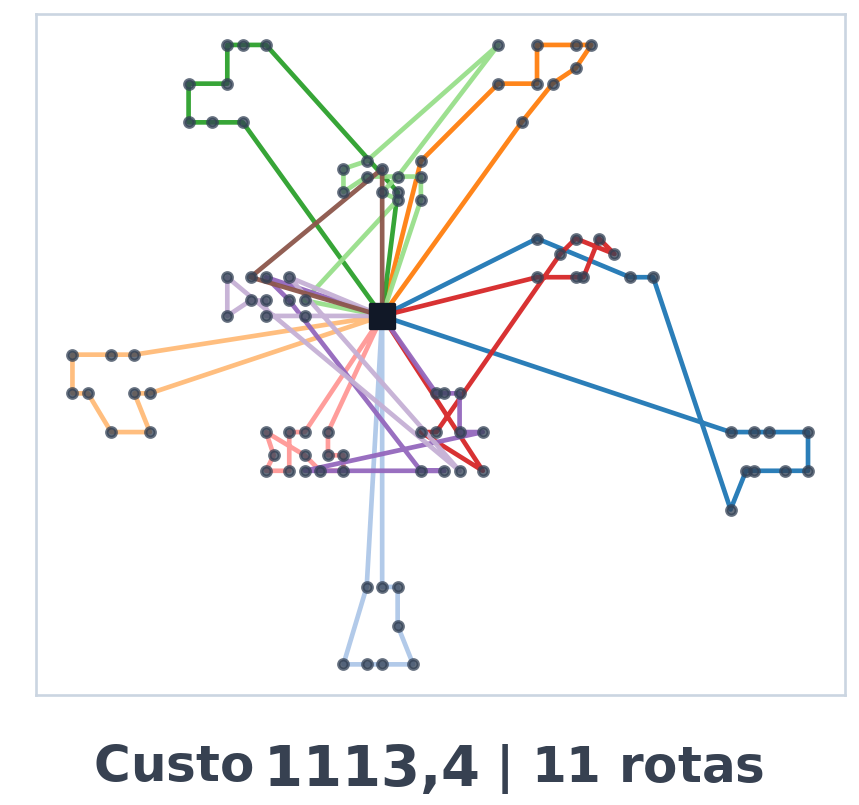
\includegraphics[width=\linewidth]{route_compare_C_panel_1}
\caption{Solomon I1}
\end{subfigure}
\hfill
\begin{subfigure}[t]{0.32\textwidth}
\centering
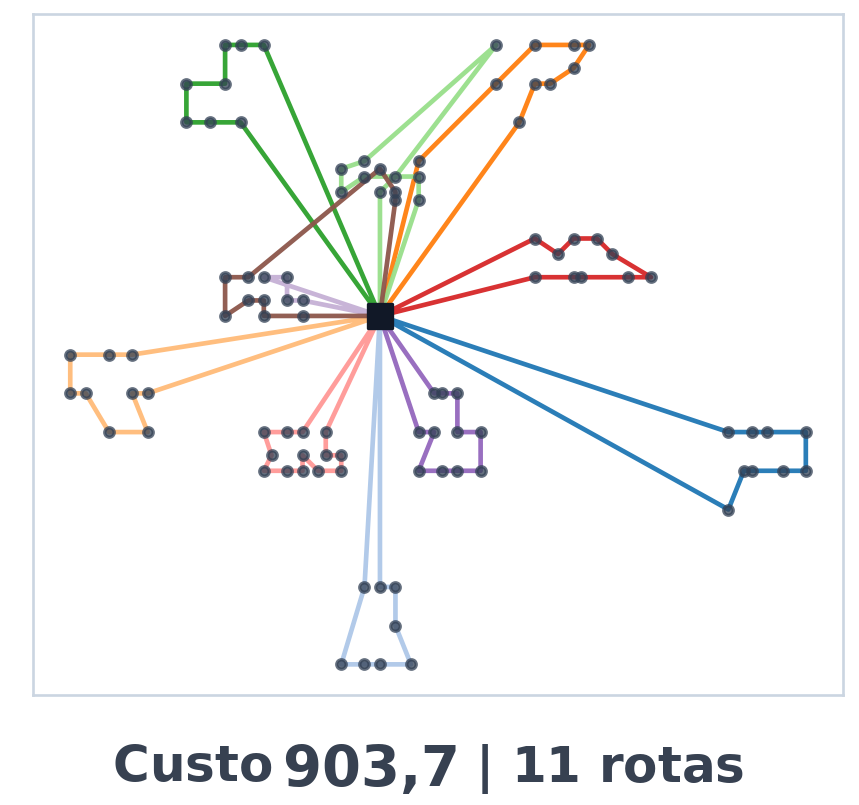
\includegraphics[width=\linewidth]{route_compare_C_panel_2}
\caption{VND}
\end{subfigure}
\hfill
\begin{subfigure}[t]{0.32\textwidth}
\centering
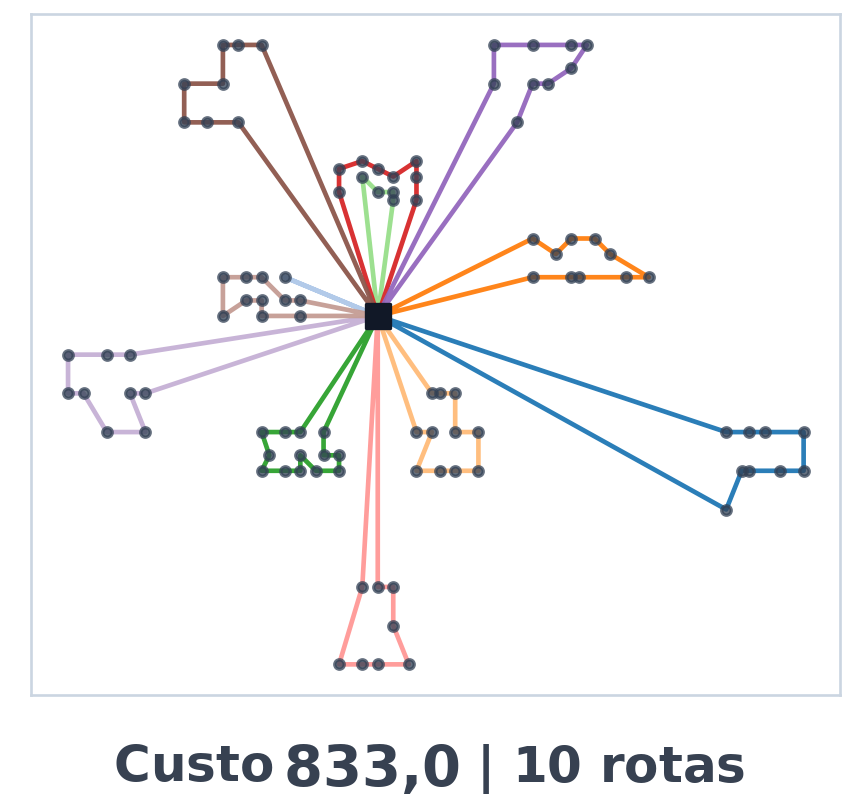
\includegraphics[width=\linewidth]{route_compare_C_panel_3}
\caption{GRASP fixo}
\end{subfigure}

\par\medskip

\makebox[\textwidth][c]{%
\begin{subfigure}[t]{0.32\textwidth}
\centering
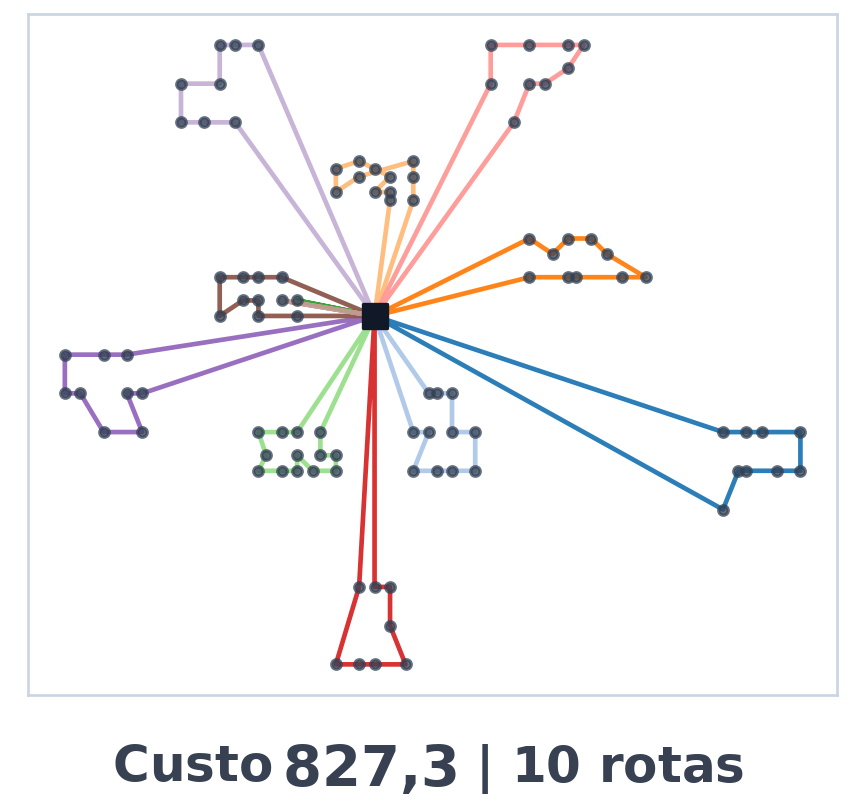
\includegraphics[width=\linewidth]{route_compare_C_panel_4}
\caption{GRASP reativo}
\end{subfigure}
\hspace{0.02\textwidth}
\begin{subfigure}[t]{0.32\textwidth}
\centering
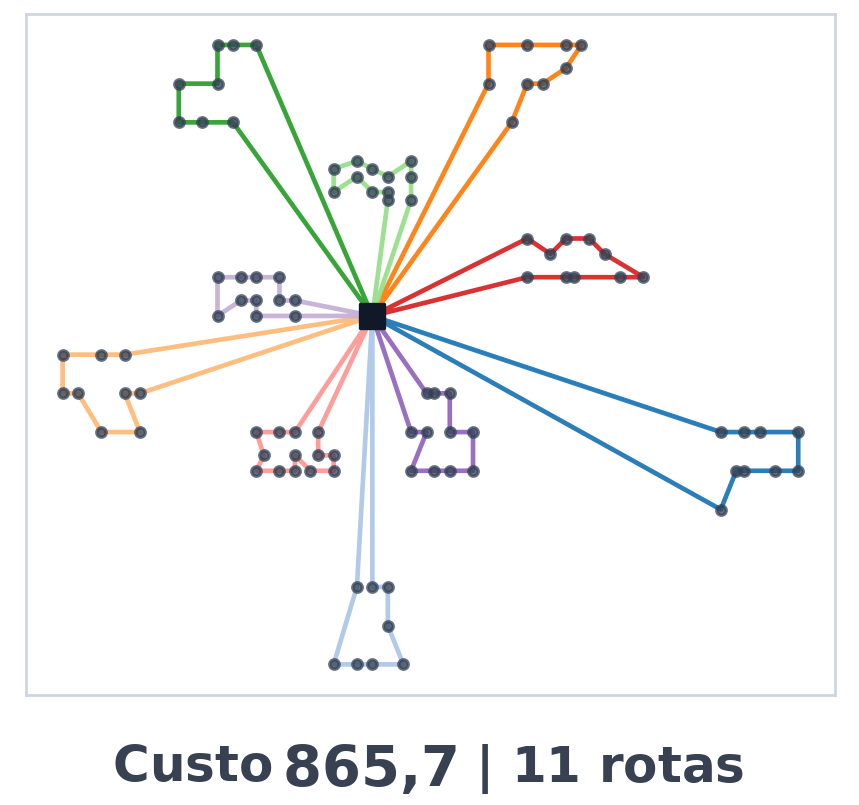
\includegraphics[width=\linewidth]{route_compare_C_panel_5}
\caption{Busca Tabu}
\end{subfigure}}
\caption*{Fonte: produ\c{c}\~ao da pr\'opria autora.}
\end{figure}

\subsection{Valida\c{c}\~ao Estat\'istica}

A compara\c{c}\~ao entre algoritmos segue o protocolo n\~ao-param\'etrico recomendado por \citet{demsar2006}: teste de Friedman sobre os \emph{ranks} de cada m\'etodo nas inst\^ancias do \emph{holdout set}, seguido pelo \emph{post-hoc} de Nemenyi com corre\c{c}\~ao para m\'ultiplas compara\c{c}\~oes. O resultado final inclui (i) o $p$-valor do Friedman, (ii) os \emph{ranks} m\'edios por m\'etodo e (iii) o diagrama de difer\c{e}n\c{c}as cr\'iticas (CD diagram). A consolida\c{c}\~ao desses indicadores ser\'a apresentada na vers\~ao final ap\'os o encerramento da Etapa~7 (testes computacionais), conforme cronograma.

\subsection{Integra\c{c}\~ao IoT--Solver: Ensaio Inicial}

A vers\~ao inicial do simulador IoT confirmou a gera\c{c}\~ao de eventos de enchimento e a comunica\c{c}\~ao com o solver via interface de arquivos. O ensaio executado verifica: (i) cria\c{c}\~ao consistente de inst\^ancias VRPTW a partir do estado dos sensores; (ii) chamada do solver com or\c{c}amento limitado de tempo; (iii) retorno das rotas ao simulador para visualiza\c{c}\~ao. A integra\c{c}\~ao completa com o Digital Twin (Etapa~6) e a valida\c{c}\~ao em escala (Etapa~7) s\~ao as pr\'oximas metas do subprojeto.

% =================================================================
\section{Conclus\~ao e Trabalhos Futuros}
\label{sec-conclusao}

Este relatório apresentou a metodologia consolidada para o desenvolvimento de um \emph{solver} VRPTW com integra\c{c}\~ao IoT, aplic\'avel \`a coleta de res\'iduos s\'olidos. Foram detalhados, em pseudoc\'odigo formal, os algoritmos implementados em C++20: Solomon I1, VND, GRASP (fixo e reativo) e Busca Tabu. A metodologia experimental adota duas conven\c{c}\~oes de objetivo (DIMACS e Solomon cl\'assico) em paralelo, com BKS provenientes do s\'itio pessoal de Solomon devido \`a indisponibilidade do reposit\'orio Gehring \& Homberger. A calibra\c{c}\~ao por irace e a valida\c{c}\~ao estat\'istica n\~ao-param\'etrica garantem rigor metodol\'ogico na compara\c{c}\~ao entre m\'etodos.

As pr\'oximas etapas do subprojeto consistem em: (a) consolidar os experimentos sobre o conjunto \texttt{holdout} ap\'os calibra\c{c}\~ao final via irace; (b) integrar o simulador IoT ao Digital Twin de visualiza\c{c}\~ao; (c) avaliar cen\'arios mais representativos da opera\c{c}\~ao real de coleta. Como extens\~oes futuras, destacam-se a incorpora\c{c}\~ao de metaheur\'isticas baseadas em popula\c{c}\~ao (HGS \citep{vidal2013}) e a utiliza\c{c}\~ao de dados reais para valida\c{c}\~ao do modelo.

\bibliographystyle{apalike}
\renewcommand{\bibsection}{\section*{Refer\^encias}}
\bibliography{referencias}

\end{document}
